\chapter{Einleitung}
\label{chap:Einleitung}

\section{MyContactCenter}
\label{sec:MyContactCenter}
In vielen Bereichen modernen Lebens hat sich seit dem Anstoß des digitalen Zeitalters ein signifikanter Wandel eingestellt. Das weite Feld  der zwischenmenschlichen Kommunikation zeigt dies wie kaum ein anderes auf. Auch an der Schnittstelle zwischen Privat- und Arbeitsleben und im Speziellen an der Kommunikation zwischen Unternehmen und ihren Kunden tritt diese Modernisierung in Erscheinung. Eine moderne Institution dieser Art der Kommunikation ist das Contact Center. Hierbei handelt es sich um einen zentralen Anlaufpunkt für Kunden, an dem diese über verschiedene Kommunikationskanäle ein Anliegen anbringen können, welches von Agenten des Unternehmens bearbeitet wird. Diese Kommunikation ist jedoch nicht einseitig: Auch Contact Center nehmen Kontakt zur Kundschaft auf, um beispielsweise Marktforschung zu betreiben. 
\newline
Laut einer Studie, die 450 Contact Center befragt hat (siehe \cite{Deloitte:17}), werden die Kommunikationsanforderungen von modernen Contact Centern nicht nur umfangreicher, sondern auch komplexer. Die von der Firma ilogixx hergestellte Software-Lösung MyContactCenter (im Folgenden mit MyCC abgekürzt) hat zum Ziel, Betreibern von Contact Center dabei zu unterstützen, diese wachsenden Anforderungen zu erfüllen. Dafür stellt das Produkt Werkzeuge zur Verfügung, die die Effizienz bei der Bearbeitung von Kundenanfragen erhöhen. Im Folgenden sollen die Elemente von MyContactCenter, die für die vorliegende Ausarbeitung relevant sind, kurz erläutert werden.

\subsection{MyContactCenter Server}
MyContactCenter ist eine verteilte Anwendung. Die Hauptkomponente dieser Anwendung ist der MyCC-Server, welcher den Großteil der Verwaltungsaufgaben übernimmt und mit den anderen MyCC-Komponenten über das Transmission Control Protocol (TCP) in Verbindung steht. Der Server verwaltet unter anderem die angemeldeten Agenten sowie Daten über ein- und ausgehende Konversationen. Eine Konversation ist im Kontext von MyCC eine Kontaktaufnahme mit dem Contact Center durch einen Endkunden über einen beliebigen Kommunikationskanal wie zum Beispiel Telefon, Email etc. Konfiguriert wird der Server über einen Administrations-Client, in welchem der Administrator des Contact Centers alle für den Betrieb benötigten Einstellungen vornehmen kann. 

\subsection{IP-Private Branch Exchange}
Die Voice-Over-IP-Technologie, über die MyCC mit Anrufern interagiert, wird nicht von MyCC selber implementiert, sondern von Drittanbieter-Software in Form einer IP-Private Branch Exchange, im Folgenden mit PBX abgekürzt. Diese ist die Software-Implementierung einer Telefonanlage, an der mehrere Teilnehmer sich mit sogenannten Soft-Phones anmelden können, um untereinander Telefonsitzungen aufzubauen. Ein Soft-Phone ist eine Software, die die Funktionen eines klassischen Telefonapparats zur Verfügung stellt. Telefonate zwischen einem Teilnehmer der PBX und einem Sitzungspartner eines anderen Netzes, also zum Beispiel einer anderen Voice-Over-IP-Anlage oder dem ISDN-Telefonnetz, laufen über eine Netzwerk-Komponente namens Gateway ab, welche die benutzten Protokolle entsprechend für den jeweils anderen Sitzungsteilnehmer umwandelt. Die mit MyCC verwendete PBX kommuniziert mit ihren Teilnehmern über das Session Initiation Protokoll, kurz SIP, welches dafür benutzt wird Kommunikationssitzungen zwischen Teilnehmern auszuhandeln. Die PBX steht mit dem MyCC-Server über eine TCP-Verbindung in Kontakt und tauscht Informationen aus, zum Beispiel welcher Agent als nächstes für eine Konversationsanfrage frei ist. 

\subsection{Agenten}
Ein Agent ist im Kontext von MyContactCenter ein Teilnehmer des Contact Centers, welcher Konversationen aufnimmt und das Anliegen der Konversation bearbeitet. Agenten besitzen eine eigene Client-Anwendung, die sich für die Dauer der Nutzungszeit am MyCC-Server anmeldet.  Mit diesem Client kann der Agent seine Konversationen durchführen, also zum Beispiel eine Email beantworten oder sein Soft-Phone, welches an der PBX angemeldet ist, über eine API steuern. Abbildung \ref{fig:MyCCStructure}  bringt zum Ausdruck, wie der MyCC-Server, die MyCC-Agenten-Clients, der MyCC-Admin-Client, die PBX und die Soft-Phones in Verbindung stehen.
\begin{figure} %[hbtp]
	\centering
		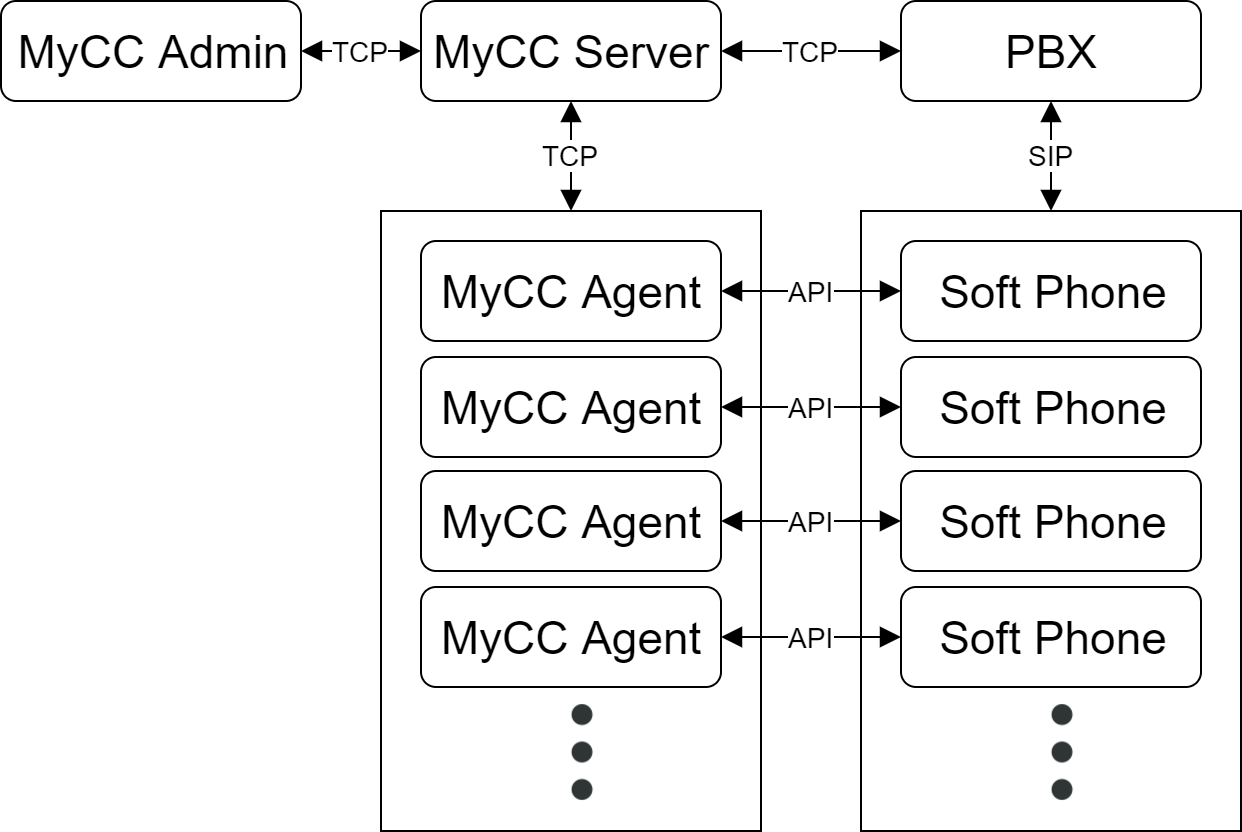
\includegraphics[width=0.8\textwidth]{img/MyCCStructure.png}
	\caption[Komponententstruktur von MyContactCenter]{Die Komponenten von MyContactCenter und wie sie miteinander in Verbindung stehen. Der MyCC-Server übernimmt eine zentrale Rolle und verwaltet die Agenten- und Admin-Clients, die über TCP mit ihm in Verbindung stehen. Die eigentliche Voice-Over-IP-Infrastruktur wird über eine PBX realisiert, an welcher die Softphones der Agenten angebunden sind. Die Schnittstelle zwischen MyCC und der PBX ist auf der Server-Seite eine TCP-Verbindung, über die Nachrichten ausgetauscht werden, und auf der Client-Seite eine API, über die der MyCC-Agent mit dem Softphone kommuniziert.}
	\label{fig:MyCCStructure}
\end{figure}
Jeder Agent besitzt eine Qualifikation in Sprachen und Wissensbereichen. Sprachen und Wissensbereiche werden vom MyCC-Administrator angelegt und bestimmen, welche Konversation ein Agent führen kann. Jeder Konversationen wird eine Sprache und ein Wissensbereich zugeteilt, sodass nur Agenten, die eine Qualifikation für diese beiden Bereiche mitbringen, die Konversation annehmen können. Zum Beispiel kann ein Agent in den Sprachen ``Englisch'' und ``Deutsch'' sowie in dem Wissensbereich ``Vertrieb'' eine Qualifikation besitzen. Dieser Agent kann Konversationen führen, denen die Sprache ``Englisch'' und der Wissensbereich ``Vertrieb'' zugeteilt ist, jedoch nicht solche, denen der Wissensbereich ``Support'' zugewiesen ist.

\newpage

\subsection{Automatische Kontaktverteilung}
Eine Kernaufgabe von MyCC ist die Automatische Kontakt Verteilung, deren englischer Fachbegriff automatic contact distribution, kurz ACD, lautet und dafür zuständig ist, eingehende Konversationen automatisch an Agenten zu verteilen. Jeder Wissensbereich besitzt eine ACD, welche Konversationen, denen dieser Wissensbereich zugewiesen wird, dem nächsten freien qualifizierten Agenten zustellt. Ist im Moment des Konversationseingangs kein Agent frei, wird diese in eine Warteschlange eingereiht und zugestellt, sobald ein qualifizierter Agent frei wird.

\subsection{Routing Engine}
In Version zehn von MyContactCenter kommt die Routing Engine als neue wichtige Software-Komponente hinzu. Diese nimmt eingehende Anrufe auf Ebene des Session Initiation Protocol (SIP) entgegen und kommuniziert an Stelle des MyCC-Servers mit der PBX. Die Routing Engine ist dafür als Teilnehmer an der PBX angemeldet und nimmt eingehende Konversationen des Contact Centers als erste MyCC-Komponente entgegen. Abbildung \ref{fig:InteractionIncomingCall} stellt den Kommunikationsablauf im Falle eines eingehenden Anrufes dar. 

\begin{figure} %[hbtp]
	\centering
		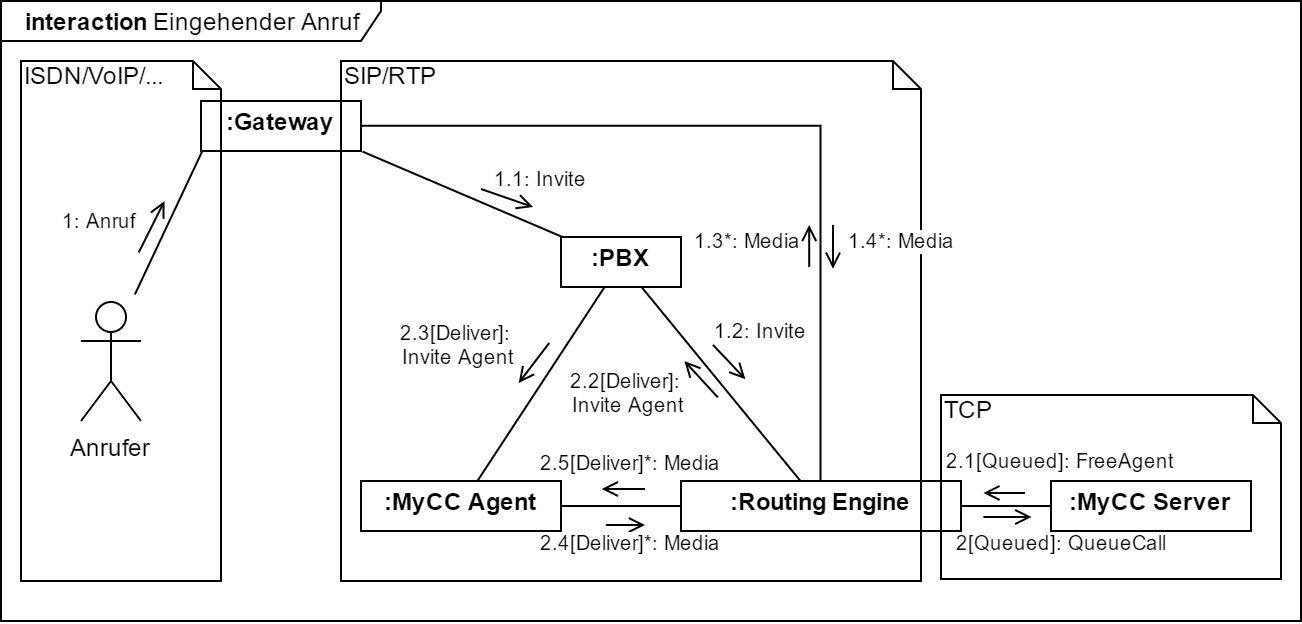
\includegraphics[width=\textwidth]{img/RoutingEngineSipExplanation.png}
	\caption[Behandlung eingehender Rufe in MyContactCenter]{Behandlung eingehender Anrufe in MyContactCenter.}
	\label{fig:InteractionIncomingCall}
\end{figure}

Ruft ein Endkunde das Contact Center an, wird über das Gateway die Schnittstelle zwischen dem anderen Telefonnetz und der PBX hergestellt. Die PBX baut über SIP eine Verbindung zur Routing Engine auf. Ist die Sitzung erfolgreich hergestellt, kann der Medienstrom zwischen dem Gateway und der Routing Engine ausgetauscht werden. Nun hat die Routing Engine Kontrolle über den Konversationsablauf und kann verschiedene Aktionen ausführen. Zum Beispiel kann ein Zustellung an einen freien Agenten über eine ACD initiiert werden. Dafür weist die Routing Engine dem Anruf einen Wissensbereich und eine Sprache zu und schickt dem MyCC-Server die Anweisung, den aktuellen Ruf in der Warteschleife einer ACD zu platzieren. Der Server antwortet mit der Information, welchem freien und qualifizierten Agenten der Ruf zugeteilt werden soll. Anschließend wird über die PBX eine Sitzung zwischen dem Agenten und der Routing Engine ausgehandelt. Die Routing Engine verschmilzt nun beide Medienströme, sodass die Medien des Agenten beim Anrufer ankommen und umgekehrt. 
\newline
Die Routing Engine hat eine hohe Kontrolle darüber, wie mit einem eingehenden Anruf umgegangen wird. So kann der Anruf zum Beispiel nicht zugestellt, sondern alternativ sofort aufgelegt werden. Auch die Manipulation des Medienstroms zwischen Anrufer und Agent ist denkbar. Die vorliegende Ausarbeitung beschäftigt sich mit dem Entwurf und der Implementierung einer domänenspezifischen Sprache, die es Benutzern von MyContactCenter ermöglicht, das Verhalten der Routing Engine frei zu spezifizieren. Die domänenspezifische Sprache dient dazu, den Ablauf aller von der Routing Engine auszuführenden Schritte zur Behandlung einer eingehenden Konversation zu modellieren. Sie wird im Folgenden entsprechend der Abkürzung des englischen Fachbegriffs ``domain-specific language'' als DSL betitelt. Ein einzelnes in der DSL verfasstes Modell, welches einen Ablauf spezifiziert, wird im Folgenden Konversationsrouting genannt.
 
\section{Motivation}
\label{sec:Motivation}
Die Motivation des vorliegenden Projektes soll zum Einstieg mit folgenden User-Stories eingeleitet werden:
\begin{itemize}
\item Als Administrator möchte ich, dass MyCC vor dem Zustellen eines Kundenrufes eine Begrüßung abspielt.
\item Als Administrator möchte ich, dass ein Anrufer die Personalnummer seines Sachbearbeiters auf der Telefontastatur eingeben kann, und an diesen weitergeleitet wird, falls dieser verfügbar ist. Andernfalls wird der Anrufer in eine Warteschlange eingereiht. 
\item Als Administrator möchte ich, dass eingehende Anrufe außerhalb der Ge\-schäftszeiten den Anrufer per Spracheinspieler darauf aufmerksam machen, und entsprechend abgelehnt werden.
\item Als Administrator möchte ich, dass MyCC bei einer eingehenden Emil mit einer Bestätigungs-Email antwortet.
\end{itemize}
Den oben aufgelisteten Anforderungen ist nicht nur die eingenommene Kundenrolle des Administrators gemeinsam. Auch die zu erreichenden Ziele ähneln sich: Die Behandlung einer eingehenden Kontaktanfrage durch die Software soll vom Kunden konfigurierbar sein. Dabei soll dem Kunden größtmögliche Freiheit geboten werden, um möglichst viele Anforderungen eines Contact Centers abzudecken. Zu den oben stehenden User-Stories können noch zahlreiche weitere Beispiele mit ähnlichem Muster konstruiert werden. Die Software MyContactCenter hat den Anspruch, all diesen Anforderungen gerecht zu werden, um in möglichst vielen Contact Centern Anwendung finden zu können. Der so resultierende Grad an individuellen Konfigurationsmöglichkeiten der Software ist hoch. Das Problem wird bewältigt, indem es dem Benutzer ermöglicht wird, das Verhalten von MyContactCenter im Falle einer Kontaktanfrage selber zu programmieren. Als Mittel dazu wird eine eigene grafische domänenspezifische Programmiersprache angeboten, deren Entwicklung und Implementierung Hauptgegenstand der vorliegenden Arbeit ist.
\newline
Für MyContactCenter als Software-Produkt ergibt sich aus diesem Vorgehen eine Reihe von Vorteilen:

\begin{description}
\item[Flexible Konfiguration] \hfill \\
Der Anwender erhält erhöhte Kontrolle über das Conversation Routing in seinem Contact Center. Die Features, die in der DSL angeboten werden sind zwar nicht neu. Aber nun kann flexibler auf diese zugegriffen werden und mehr Anforderungen von Contact Centern können erfüllt werden.
\item[Unabhängigkeit gegenüber Drittanbietern] \hfill \\
Vor der Implementierung der DSL lief das Conversation Routing über die PBX ab: Eingehende Anrufe wurden über eine Scripting-Schnittstelle der Telefonanlage geroutet. Mit einer eigenständigen DSL erhält MyCC eine neue Unabhängigkeit gegenüber den Beschränkungen und Nachteilen solcher Drittanbieter-Software.
\item[Hohe Skalierbarkeit] \hfill \\
Die Ausführung von DSL-Skripten wird von einem dediziertem Dienst, der Routing Engine, übernommen. Dies entlastet den MyCC-Server und erlaubt das parallele Aufschalten von mehreren Conversation Routing Engines bei hoher Systemlast. So kann die allgemeine Performanz von MyCC verbessert werden.
\end{description}

\section{Domänenspezifische Sprachen}
Bei domänenspezifischen Sprachen handelt es sich um formale Sprachen, die es einem menschlichen Benutzer ermöglichen, Programmabläufe zu spezifizieren. In diesem Punkt ähneln sie prominenten Programmiersprachen wie C oder Java. Anders als diese Universalsprachen (engl. General Purpose Languages), welche Turing-vollständig sind, werden DSLs jedoch absichtlich mit beschränktem Anwendungsgebiet designt. Ihre Anwendung beschränkt sich auf das Lösen von Problemen aus einer bestimmten Domäne. Diese Domänen können vielfältig sein: Beispiele sind hier das Steuern von Kühlschränken, das Spezifizieren von Benutzeroberflächen von Handy-Anwendungen oder das Beschreiben von Versicherungspaketen (siehe \cite[S. 93ff.]{Kelly:08}. Besondere Beachtung finden DSLs in der modellgetriebenen Softwareentwicklung (engl. Model Driven Devlopment oder MDD), welche zum Ziel hat, Software nicht mehr über herkömmlichen, von Hand geschriebenen Quellcode zu entwickeln. Stattdessen wird Software in Form von Modellen spezifiziert, welche in einer oftmals eigens für das Problem entworfenen DSL ausgedrückt werden. Diese Modelle werden als Vorlage genommen, um daraus ausführbaren Code, oft in einer  Universalsprache, zu generieren \cite[S. 29]{Voelter:13}. Dies wird als Transformation bezeichnet. Der Fokus beim Model Driven Development liegt also nicht mehr auf dem Quellcode selbst, sondern auf Modellen, welche das Verhalten der Software spezifizieren \cite[S. 3]{Kleppe:09}. Befürworter von domänenspezifischen Sprachen loben den Einsatz solcher als Mittel, um die Qualität der entstehenden Software und die Produktivität des Herstellungsprozesses zu erhöhen \cite[S. 33f]{Fowler:11}. Die Transformation eines DSL-Modells in Code einer maschinennäheren Programmiersprache sei vergleichbar mit dem Sprung auf höhere Abstraktionsstufen, der vollzogen wird, wenn Programmiersprachen einen Generationswechsel vollziehen. Damit einher gingen die verbundenen Vorteile bei der Softwareentwicklung \cite[S. 15ff]{Kelly:08}.
\newline
In der vorliegenden Arbeit wird eine domänenspezifische Sprache nicht im Zuge von modellgetriebener Softwareentwicklung eingesetzt, denn die Anwender der Sprache verwenden diese nicht mit dem Ziel, Software-Produkte für andere Benutzer zu entwickeln. Stattdessen spezifiziert die DSL das Verhalten einer einzelnen Komponente von MyCC und wird ausschließlich in diesem Kontext eingesetzt. Eine domänenspezifische Sprache bietet sich für diese Aufgabe aus folgenden Gründen an: 
\begin{description}
\item[Modellierung statt Programmierung] \hfill \\
Bei der Zielgruppe der DSL handelt es sich nicht um Programmierer, sondern um Anwender von MyContactCenter. Die Anwender sind versiert im Betreiben eines Contact Centers und haben ein breites Wissen über die Domäne: Das Routing von Konversationen in Contact Centern. Es handelt sich um sogenannte Domänenexperten (engl. domain experts). Es kann jedoch nicht davon ausgegangen werden, dass Domänenexperten über Programmierkenntnisse mit Universalsprachen verfügen. Würde eine solche Universalsprache zum Einsatz kommen, bestünde ein Risiko, dass ein großer Teil der Zielgruppe aufgrund von fehlender Qualifizierung und Verständnis das Produkt nicht nutzen kann. Ebenso werden Anwender vor fehlerhafter Programmierung geschützt. Dies ist auch der Grund, warum eine grafische und keine textuelle DSL zum Einsatz kommt: Grafische Repräsentationen gelten laut \cite[S. 50f]{Kelly:08} als ausdrucksstärker, verständlicher und weniger fehleranfällig.
\item[Domänenspezifische Einschränkung] \hfill \\
Die Anzahl an unterschiedlichen Möglichkeiten zur Konfigurierung des Konversationsroutings rechtfertigt deren Programmierbarkeit. Dennoch muss hier keine Turing-vollständige Programmierung stattfinden. Durch die Einschränkung auf eine Domäne profitiert der Anwender von den Vorteilen, die domänenspezifische Sprachen zugeschrieben werden: Weniger Fehler mit aussagekräftigeren Fehlermeldungen, sicherere und leichter zu analysierende Programme sowie leichtere Erlernbarkeit \cite{Tomassetti:17}.
\item[Verbesserte Kommunikation] \hfill \\
Als Benutzer von MyContactCenter stehen die Anwender der DSL häufig in Kontakt mit dem Hersteller (beispielsweise im Zuge von technischem Support oder bei Verkaufsgesprächen). In diesen Austauschen ist eine eindeutige Kommunikation wichtig, auch wenn es um das Routing von Konversationen geht. Die grafischen Modelle der DSL stellen eine unmissverständliche Dokumentation der Spezifikation solcher Konversationsroutings dar, die sowohl aus Entwickler- als auch aus Domänenexpertensicht verständlich ist. Auf diese Weise trägt die DSL zur erfolgreichen Kommunikation zwischen Anwendern und dem Hersteller bei.
\end{description}


\section{Benötigtes Vorwissen}
MyContactCenter kommt in einem umfangreichen Ökosystem von Drittanbieter-Software zum Einsatz. Für das weitere Verständnis der vorliegenden Arbeit werden die Prinzipien einiger Technologien und Themen erläutert, welche Einfluss auf die Implementierung der domänenspezifischen Sprache nehmen. 

\subsection{.NET}
MyContactCenter und die DSL ist mit dem Microsoft .NET Software Framework entwickelt worden. Hauptbestandteile von .NET ist die Microsoft Intermediate Language (MSIL), auch genannt Common Intermediate Langugage (CIL), und die Common Language Runtime (CLR), welche Sprachinteroperabilität zwischen unterschiedlichen Universalsprachen (wie zum Beispiel C\# oder Visual Basic) ermöglicht. Benutzer des .NET Frameworks schreiben Code in einer vom Framework unterstützen Sprache, welcher vom Compiler in MSIL-Bytecode übersetzt wird. Dieser Bytecode wird von der CLR mittels eines Just-In-Time-Compilers in Maschinencode transformiert und ausgeführt (vgl. \cite[S. 16ff]{Platt:03}). Zusätzlich stellt das .NET Framework eine große Anzahl an Bibliotheken mit grundlegenden Funktionen zur Verfügung. 

\subsection{Roslyn}
Roslyn ist eine .NET Compiler-Plattform welche Entwicklern die Werkzeuge eines Compilers für C\#- und Visual Basic-Code über eine API im eigenen Programmcode zur Verfügung stellt. So kann Code analysiert, generiert und kompiliert werden (siehe dazu den frei zugänglichen Quellcode und die Dokumenation \cite{Roslyn}). Die Implementierung der domänenspezifischen Sprache benutzt Roslyn, um über eine Codegenerierungs-API einen MSIL-Syntaxbaum zu generieren und diesen zu einem .NET-Bytecode-Assembly zu kompilieren. Über die API können einem bestehenden Syntaxbaum neue Syntaxknoten hinzugefügt werden, welche sich nach den Regeln der Microsoft Intermediate Language schachteln lassen. Syntaxknoten und -Bäume sind unveränderlich (engl. immutable), das heißt wenn ein Syntaxbaum einmal angelegt ist, kann dieser nicht mehr verändert, sondern nur noch kopiert werden. In der vorliegenden Ausarbeitung wird der Syntaxbaum mit Roslyn daher ''Bottom-up`` generiert: Anstatt zuerst den Syntaxbaum zu instanzieren und anschließend die Knoten und Baumblätter hinzuzufügen, werden zuerst die Blätter und Knoten erzeugt, welche nacheinander zu einem Baum zusammengesetzt werden. Sei beispielsweise die Syntax für folgenden Code zu generieren:
\noindent
\begin{lstlisting}[language=custom]
public class RoslynTest
{
    public int Return5()
    {
        return 2 + 3;
    }
}
\end{lstlisting}

Dann ließe sich dies durch folgenden Code-Ausschnitt realisieren:
\noindent
\begin{lstlisting}[language=custom]
var workSpace = new AdhocWorkspace();

var generator = SyntaxGenerator(workSpace, LanguageNames.CSharp);

var literal2 = generator.LiteralExpression(2);

var literal3 = generator.LiteralExpression(3);

var addExpression = generator.AddExpression(literal2, literal3);

var returnStatement = generator.ReturnStatement(addExpression);

var returnType = generator.TypeExpression(SpecialType.System_Int32);

var methodDeclaration = generator.MethodDeclaration("Return5", null, null, returnType, Accessibility.Public, DeclarationModifiers.None, returnStatement);

var methodDeclarationArray = new SyntaxNode[] { methodDeclaration };

var classDeclaration = generator.ClassDeclaration("RoslynTest", null, Accessibility.Public, DeclarationModifiers.None, null, null, methodDeclarationArray);

var classDeclarationArray = new SyntaxNode[]{ classDeclaration };

var tree = generator.CompilationUnit(classDeclarationArray).SyntaxTree;
\end{lstlisting}

\vskip 1em

\subsection{Asynchrone Methodenausführung in .NET}
\label{subsec:Asynchrone Methodenausfuehrung}
Einige Operationen innerhalb eines Konversationsroutings müssen den Ablauf dieses Routings für eine gewisse Dauer anhalten, bevor die nächste Operation ausgeführt werden kann. Zum Beispiel beim Abspielen einer Audiodatei wird das Konversationsrouting nicht fortgeführt, bis die Audiodatei nicht zu Ende ist. Die Umsetzung solcher Operationen im Quellcode  der Transformation blockiert den Programmfluss jedoch nicht, da diese Operationen mittels asynchroner Methodenausführung auf anderen Threads ausgeführt werden. Dies findet in .NET über das Async/Await-Sprachkonstrukt statt, welches anhand des unten stehenden Codes erklärt wird.
\noindent
\newline
\begin{lstlisting}[language=custom]
async Task<int> A ()
{
	int temp = await B();
	return temp;
}

Task<int> B ()
{
	return Task.Run<int>( () => DoWork() );
}
\end{lstlisting}

Eine Methode, hier genannt Methode \texttt{A}, kann mit dem Schlüsselwort \texttt{async} gekennzeichnet werden. Dies signalisiert, dass \texttt{A} eine asynchrone Methode ist, welche in ihrem Methoden-Körper mittels des \texttt{await}-Schlüsselworts auf die andere Methode \texttt{B} warten kann. Trifft der Programmfluss auf dieses \texttt{await}, wird die Kontrolle an den Aufrufer von \texttt{A} zurückgegeben, während auf das Ergebnis von \texttt{B} gewartet wird. Der Aufrufer von \texttt{A} kann nun mit seiner Arbeit weitermachen, oder gemäß des Musters mittels \texttt{await} auf \texttt{A} warten. \texttt{B}s Arbeit wird mit der Methode \texttt{Task.Run} gestartet, welche die zu verrichtende Arbeit auf einem anderen Thread startet und ein \texttt{Task}-Objekt zurückgibt. Ein Thread repräsentiert einen weiteren Programmablauf, welcher im aktuellen Prozess nebenläufig zu anderen Programmabläufen ausgeführt wird. Ein \texttt{Task}-Objekt bildet eine auszuführende Aufgabe ab, die asynchron zum aktuellen Hauptthread des Programmes abläuft. Ist der mit \texttt{Task.Run} gestartete Thread mit seiner Arbeit fertig (in diesem Fall mit der Methode \texttt{DoWork}) wird das Ergebnis in dem \texttt{Task}-Objekt gespeichert, von dem \texttt{await}-Operator abgeholt, und in die Variable \texttt{temp} geschrieben. \texttt{temp} wird nun zurückgeliefert, sodass das von A zurückgelieferte \texttt{Task}-Objekt nun das gewünschte Ergebnis enthält. Auf diese Weise wurde der Hauptprogrammfluss nicht blockiert, obwohl eine potentiell rechenintensive Operation in \texttt{B} ausgeführt wurde.

\subsection{SIP}
Die Kommunikation der Routing Engine mit der PBX findet über das Session Initiation Protocol statt. Es handelt sich hierbei um ein Klartext-Protokoll, welches in der Anwendungsschicht des OSI-Modells angesiedelt ist. Es wird dafür benutzt, Kommunikationssitzungen zwischen sogenannten User Agents zu initiieren. Solche User Agents können beispielsweise Soft-Phones sein, die an der PBX angemeldet sind. Die PBX agiert im Kontext von SIP als Proxy-Server, welcher die Vermittlung zwischen User Agents sicherstellt. Ist eine Kommunikationssitzung zustande gekommen, wird ein Medienstrom über das Real-Time Transport Protocol ausgetauscht. Die Routing Engine, also der Teil von MyContactCenter, der die DSL-Modelle ausführt, ist als User Agent an der PBX angemeldet und der Sitzungspartner einer eingehenden Konversation während des Verlaufs eines Konversationsroutings. Die Implementierung des Session Initiation Protocols ist an einer Drittanbieter-Bibliothek namens PJSIP ausgelagert. Diese übernimmt auch die Implementierung eines SIP User Agents. 

\subsection{Protocol Buffers}
Protocol Buffers sind eine von Google entwickelte Methode, um Daten zu serialisieren. Im hier beschriebenen Projekt wird eine Implementierung dessen namens Protobuf verwendet, um DSL-Strukturen als Bytestrom zwischenzuspeichern und zu übermitteln. Gegenüber Klartext-Verfahren wie XML oder JSON bietet Protobuf einen Performance-Vorteil (siehe \cite{Bowden:14}).

\subsection{Windows Forms und Devexpress}
Die grafische Benutzeroberfläche von MyCC und damit auch des grafischen DSL-Editors ist mit der Windows Forms-Technologie implementiert. Dabei handelt es sich um eine .NET-Bibliothek, die Werkzeuge zum Designen und Darstellen von grafischen Benutzeroberflächen zur Verfügung stellt. Obwohl es neuere Frameworks zur Entwicklung von grafischen Benutzeroberflächen gibt (zum Beispiel die Windows Presentation Foundation), werde Windows Forms laut Microsoft weiterhin unterstützt und gewartet (siehe \cite{Allen:14}). Programme die Windows Forms verwenden, benutzen zur Interaktion mit der Benutzeroberfläche .NET Events \cite[S. 171ff]{Platt:03}. Das heißt, dass die grafische Benutzeroberfläche aus Komponenten (sog. Controls) zusammengestellt wird, welche bei Interaktion durch einen Benutzer Events auslösen, auf die zu Grunde liegender Code dann reagieren kann. Zur Ergänzung von Windows Forms wird in der vorliegenden Arbeit die Drittanbieter-Bibliothek Devexpress verwendet, welche Erweiterungen vor allem in Form von komplexen Controls zur Verfügung stellt. 

\subsection{Abstrakte und konkrete Syntax}
Im Bereich der Entwicklung von formalen Sprachen wird bei der Syntax einer Sprache oft zwischen abstrakter und konkreter Syntax unterschieden. Die abstrakte Syntax eines Programmes ist eine Repräsentation in Form einer Datenstruktur, welche die semantisch relevanten Informationen enthält (nach \cite[S. 26]{Voelter:13}). Bei Text-basierten Sprachen nimmt diese Datenstruktur oftmals die Form eines Baums an, der dann als abstrakter Syntaxbaum (engl. abstract syntax tree, kurz AST) bezeichnet wird. Die abstrakte Syntax enthält keine Informationen über die visuelle Darstellung der Programm-Syntax. Stattdessen sind diese in der konkreten Syntax enthalten, welche die Form annimmt, in der ein Endbenutzer ein Programm schreibt oder modelliert. Die Syntax eines Programmes kann auf viele verschiedene Arten und Weisen visualisiert werden, beispielsweise über Text oder eine grafische Repräsentation. Daher ist es für eine Sprache möglich, mehrere konkrete Syntaxen zu haben (vgl. \cite[S. 6f]{Kleppe:09}.